\documentclass{article}
\usepackage{tikz}
\usepackage{geometry}
\usepackage{amsmath}
\usepackage{wasysym}
\usetikzlibrary{mindmap}
\geometry{a2paper, landscape, margin=2in}

\begin{document}
\begin{figure}\centering

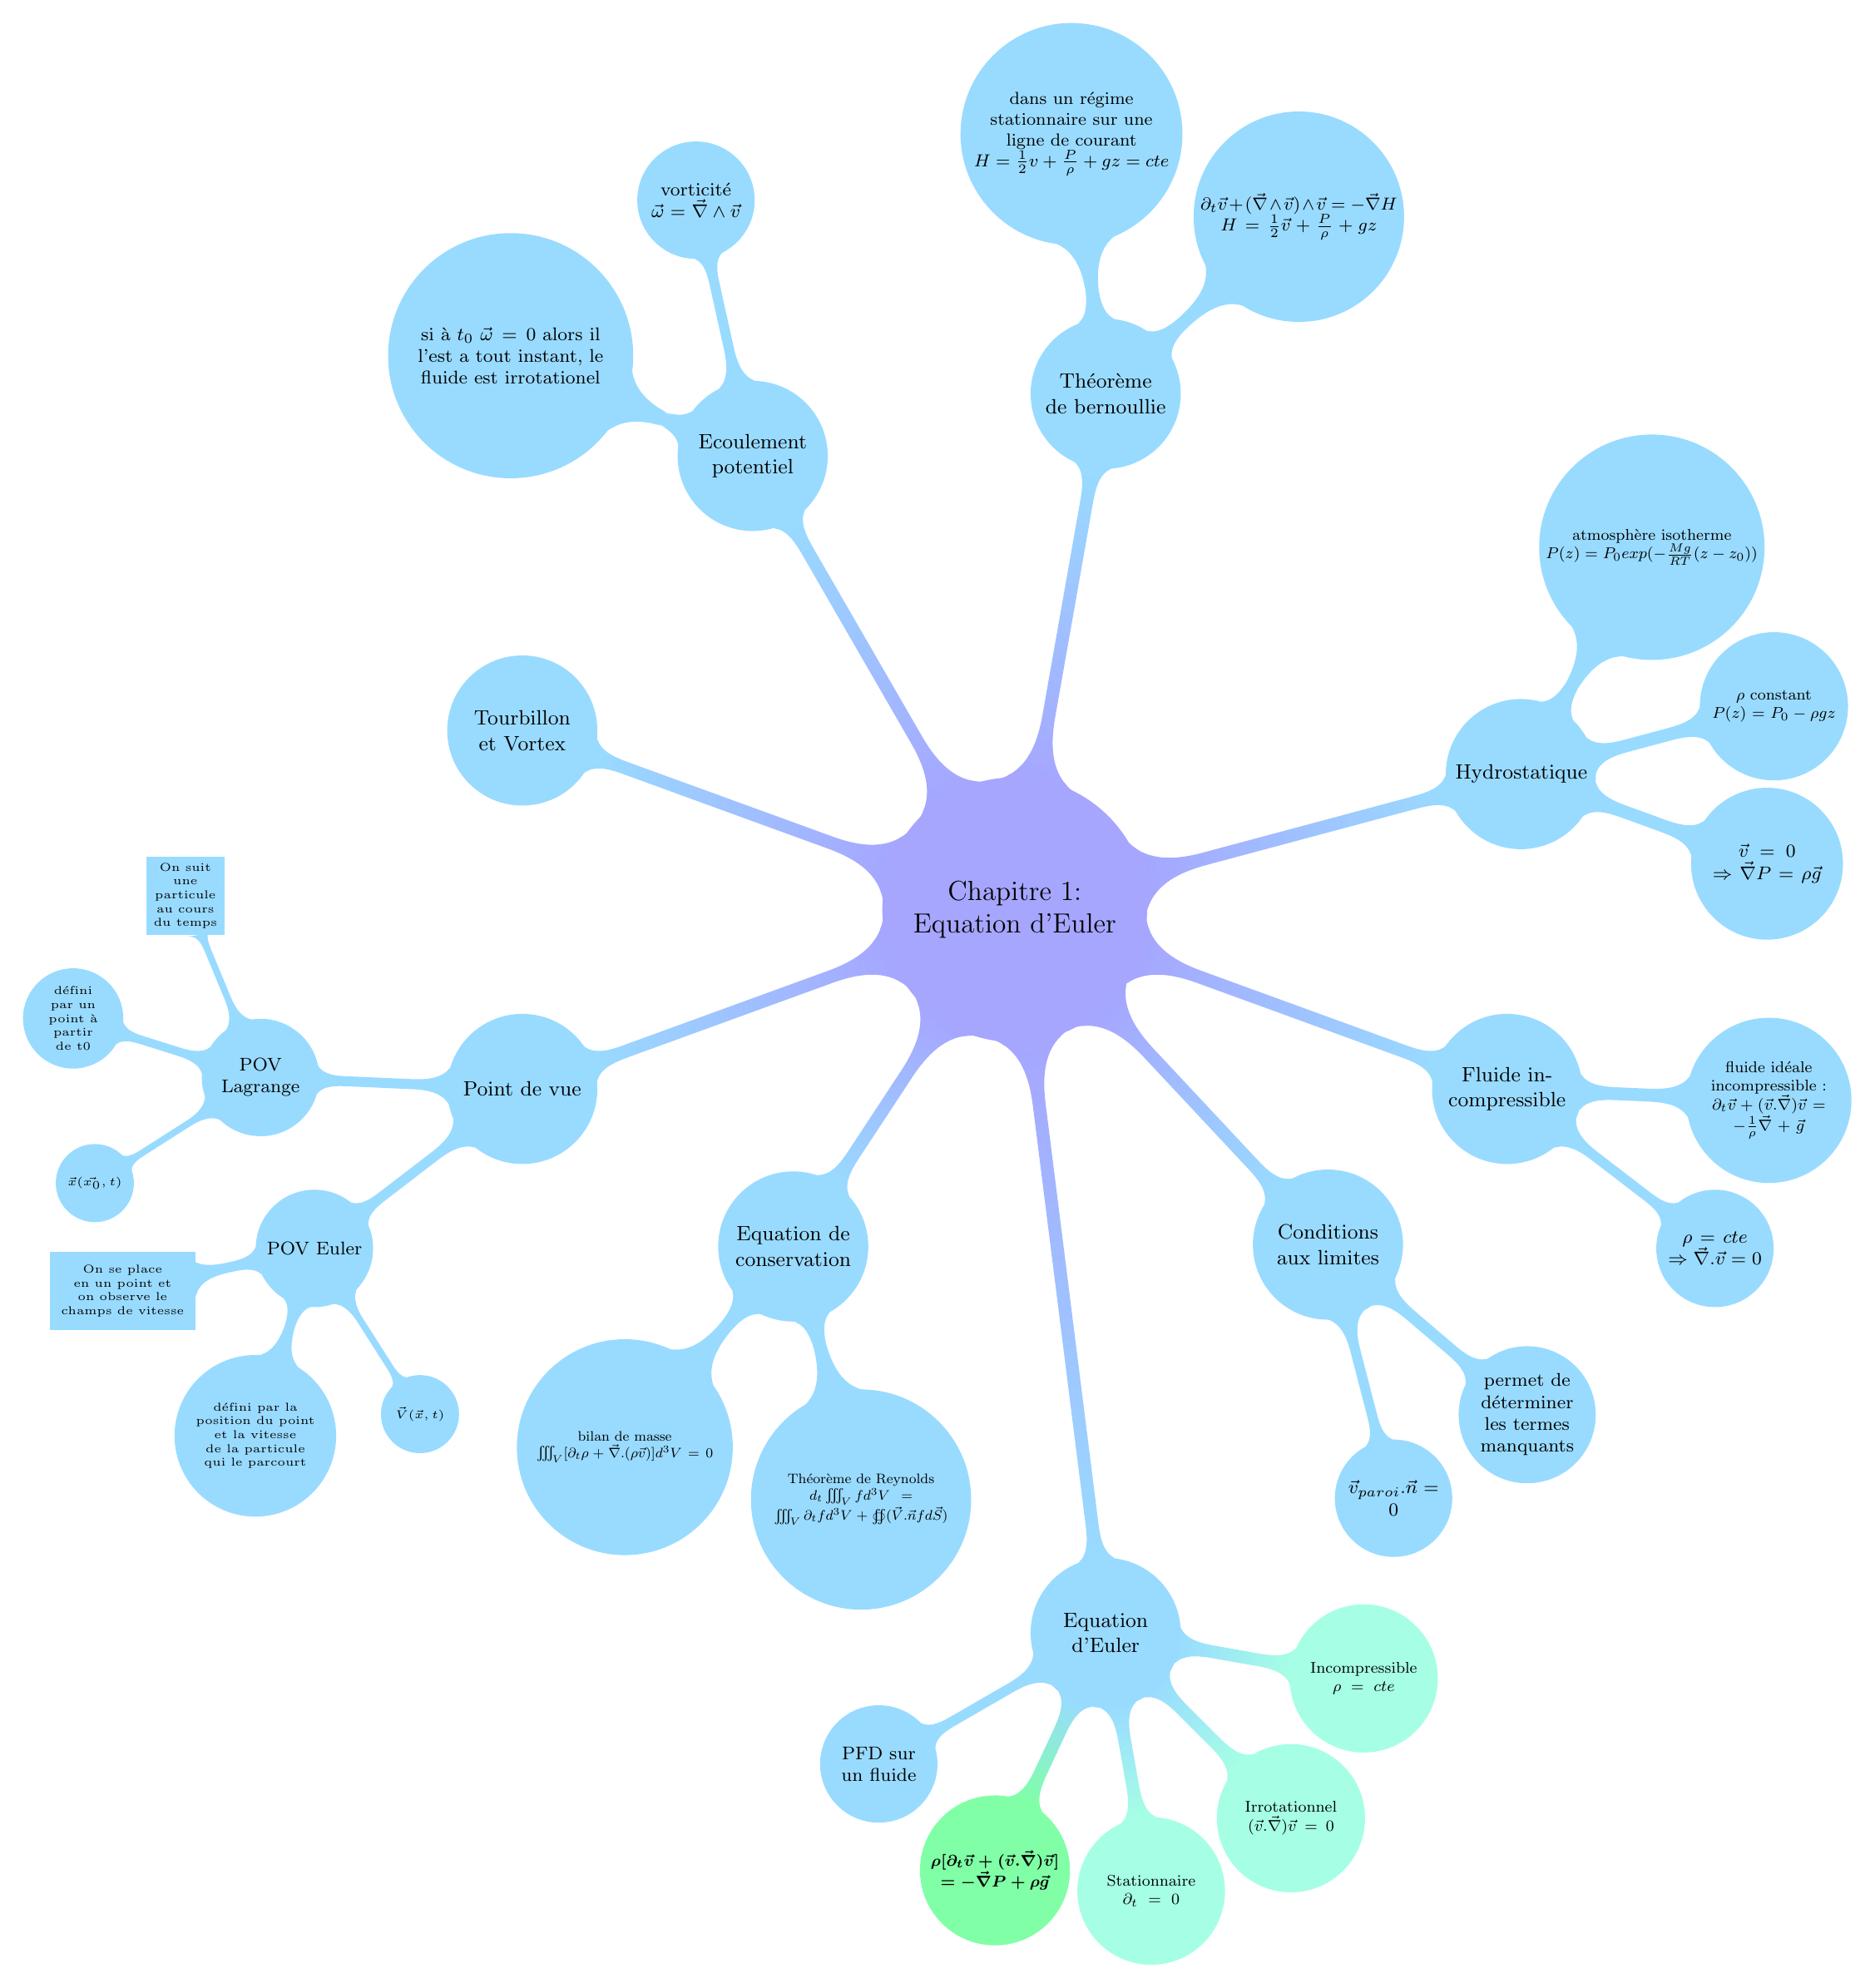
\begin{tikzpicture}[mindmap, grow cyclic, every node/.style=concept,concept color=blue!35,
	level 1/.append style={level distance=8cm,sibling angle=40,every child/.style={concept color=blue!35!cyan!40}},
	level 2/.append style={level distance=4cm,sibling angle=35},
    level 3/.append style={level distance=3cm,sibling angle=45}
    ]

\node {Chapitre 1: Equation d'Euler}
    child { node {Point de vue}
        child [rotate=-5]{node[concept] {POV Lagrange}
            child [grow=-65]{node[rectangle] {On suit une particule au cours du temps}}
            child [grow=-15]{node[concept] {défini par un point à partir de t0}}
            child [grow=35]{node[concept] {$\vec{x}(\vec{x_0},t)$}}
        }
        child {node[concept] {POV Euler}
            child [grow=-25]{node[text width=6em,text centered,rectangle]{On se place en un point et on observe le champs de vitesse}}
            child [grow=35]{node[concept,text width=6em,text centered]{défini par la position du point et la vitesse de la particule qui le parcourt}}
            child [grow=85]{node[concept]{$\vec{V}(\vec{x},t)$}}
        }
    }
    child [rotate=5]{ node[yshift=60pt]{Equation de conservation}
        child [grow=-15]{node[text width=12em,text centered,scale=.75] {bilan de masse $\iiint_V [ \partial_t\rho+\vec{\nabla}.(\rho\vec{v})]d^3V=0$}
        }
        child [grow=40]{node[text width=12em,text centered,scale=.75] {Théorème de Reynolds $d_t\iiint_V fd^3V=\iiint_V\partial_t f d^3V+\oiint (\vec{V}.\vec{n}f d\vec{S})$}
        }
    }
    child { node[yshift=-90pt]{Equation d'Euler}
        child {node[concept] {PFD sur un fluide}
            }
        child [concept color=green!70!cyan!50]{node[concept,text width=7em,text centered,scale=.85] {$\boldsymbol{\rho [ \partial_t \vec{v}+(\vec{v}.\vec{\nabla})\vec{v}]}$\\$\boldsymbol{=-\vec{\nabla}P+\rho \vec{g}}$}
        }
        child [concept color=green!30!cyan!35]{node[concept,text width=7em,text centered,scale=.85] {Stationnaire $\partial_t=0$}
        }
        child [concept color=green!30!cyan!35]{node[concept,text width=7em,text centered,scale=.85] {Irrotationnel $(\vec{v}.\vec{\nabla})\vec{v}=0$}
        }
        child [concept color=green!30!cyan!35]{node[concept,text width=7em,text centered,scale=.85] {Incompressible $\rho=cte$}
        }
    }
    child [rotate=-18,yshift=50]{ node {Conditions aux limites}
        child [concept]{node[concept] {$\vec{v}_{paroi}.\vec{n}=0$}
            }
        child [concept]{node[concept] {permet de déterminer les termes manquants }
            }
    }
    child [rotate=-20]{ node {Fluide incompressible}
        child [concept]{node[concept] {$\rho=cte$\\$\Rightarrow\vec{\nabla}.\vec{v}=0$}
            }
        child [concept]{node[concept,text width=7em,text centered,scale=.85] {fluide idéale incompressible : $\partial_t\vec{v}+(\vec{v}.\vec{\nabla})\vec{v}=-\frac{1}{\rho}\vec{\nabla}+\vec{g}$}
            }
    }
    child[rotate=-25] { node {Hydrostatique}
        child [concept]{node[concept,text width=6em,text centered] {$\vec{v}=0$\\$\Rightarrow\vec{\nabla}P=\rho \vec{g}$}
            }
        child [concept]{node[concept,text width=7em,text centered,scale=.85] {$\rho$ constant $P(z)=P_0-\rho g z$}
        }
        child [rotate=10]{node[concept,text width=11em,text centered,scale=.85] {atmosphère isotherme $P(z)=P_0 exp(-\frac{Mg}{RT}(z-z_0))$}
        }
    }
    child { node {Théorème de bernoullie}
        child[rotate=-20]{node[concept,text width=9em,text centered,scale=.95]{$\partial_t\vec{v}+(\vec{\nabla}\wedge\vec{v})\wedge\vec{v}=-\vec{\nabla}H$ $H=\frac{1}{2}\vec{v}²+\frac{P}{\rho}+gz$}
        }
        child[concept]{node[concept,text width=9em,text centered,scale=.95]{dans un régime stationnaire sur une ligne de courant $H=\frac{1}{2}v²+\frac{P}{\rho}+gz=cte$}
        }
    }
    child { node {Ecoulement potentiel}
        child[concept]{node[concept]{vorticité $\vec{\omega}=\vec{\nabla}\wedge \vec{v}$}
        }
        child[concept,rotate=20]{node[concept,text width=10em,text centered]{si à $t_0$ $\vec{\omega}=0$ alors il l'est a tout instant, le fluide est irrotationel}
        }
    }
    child { node {Tourbillon et Vortex}
    }

;


\end{tikzpicture}
\end{figure}
\end{document}